% Filename: Methods.tex
% Last update: Monday, 11/5/2018 by Ally Warner
%%%%%%%%%%%%%%%%%%%%%%%%%%%%%%%%%%%%%%%%%%%%%%%%%%%%%%%%%%%%%%%%%%%%%%

\section{Methods}
\label{sec:Methods}

%%Pipeline figure
\begin{figure}[H]
    \centering
    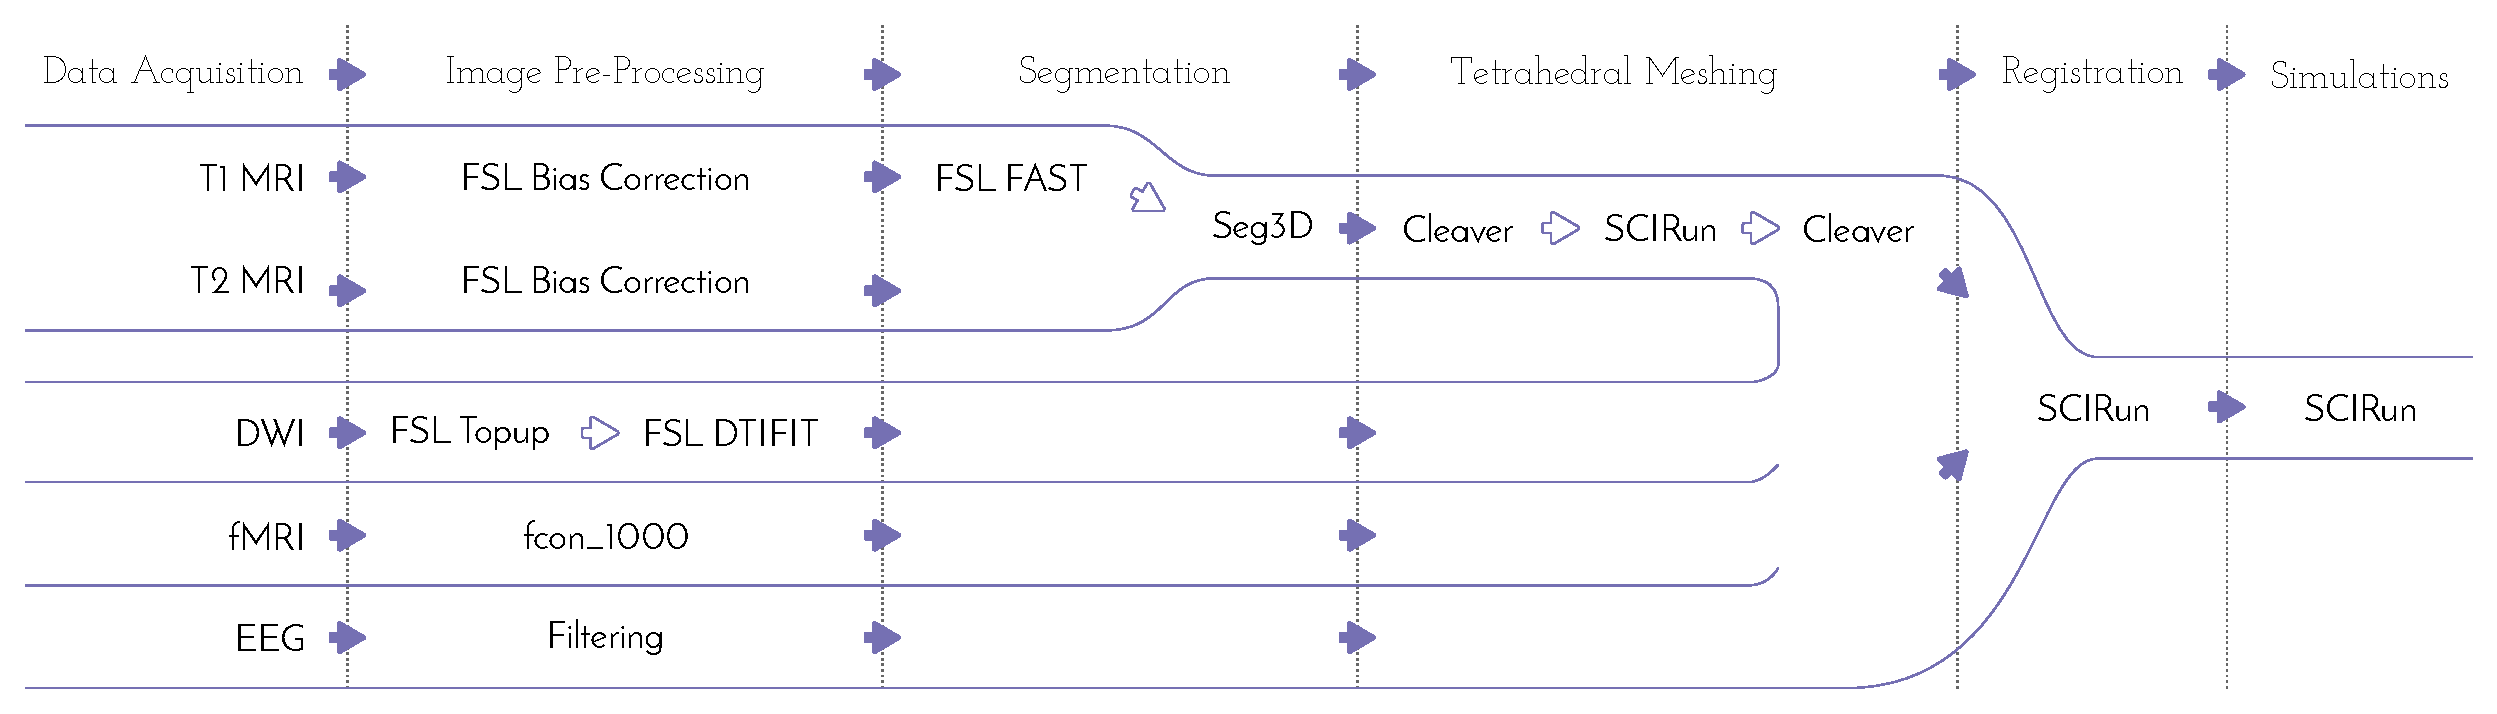
\includegraphics[width=\textwidth]{Figures/pipeline}
    \caption{Comprehensive head/brain model pipeline. Data sources are shown on the left with software packages used for creating the head/brain model in the middle and the simulation software on the right.}
    \label{fig:pipeline}
\end{figure}

\subsection{Data Acquisition}
\label{sec:Data}

%%% Image and EEG Acquisitions 

To construct a high-resolution, personalized, anisotropic volume conductor whole-head model, $T_1$-, $T_2$- weighted, diffusion weighted, and functional magnetic resonance images (MRI) were acquired on a healthy, female subject, 23 years of age, on a Skyra 3T full-body scanner (Siemens Medical Solutions, Erlangen, Germany).

The $T_1$-weighted scan was performed with a three-dimensional magnetization-prepared, rapid gradient echo (MPRAGE) sequence \cite{ref:mprage}. The parameters used were as follows: echo time: 3.41ms; repetition time: 2500ms; flip angle: 7 $^{\circ}$; resolution matrix size: 256x256 pixels; field of view: 256mm; 208 sagittal slices with a slice thickness of 1mm. Acquisition time was 10:42 minutes.

The $T_2$-weighted scan was performed with a SPACE - sampling perfection with application-optimized contrast using different flip angle evolutions - sequence \cite{ref:space}. The parameters used were as follows: echo time: 406ms; repetition time: 3200ms; resolution matrix size: 256x256 pixels; field of view: 256mm; 208 sagittal slices with a slice thickness of 1mm. Acquisition time was 5:34 minutes. The subject did not move in between the two scans so the scans did not need to be registered.

The diffusion weighted images (DWI) were acquired with multiband two-dimensional echo-planar imaging (EPI) \cite{ref:epi}. Both phase encoding directions were performed (anterior to posterior and posterior to anterior) with 64 diffusion directions each. Further sequence parameters for each scan were as follows: echo time: 76.8ms; repetition time: 4070ms; flip angle: 90 $^{\circ}$; resolution matrix size: 104x104 pixels; field of view: 208mm; 60 slices with 2.5mm slice thickness. Acquisition time was 5:05 minutes each.

The functional MRI (fMRI) scans were acquired with a blood oxygenation level dependent contrast (BOLD) sequence. The following parameters were used: echo time: 76.8ms; repetition time: 780ms; flip angle: 55 $^{\circ}$; resolution matrix size: 104x104 pixels; field of view: 210mm; 72 slices with 2mm slice thickness. Acquisition time was 10:32 minutes.

Multiple continuous electroencephalograms (EEGs) was recorded using both a 128-channel and 256 channel HydroCel Geodesic Sensor Net that was connected to a NetAmps 400 amplifier and referenced online to a single vertex electrode. Channel impedances were kept at or below 50 kOhms and signals were sampled at 250Hz. The EEGs were recorded while the subject sat quietly in a chair, alternating two-minute epochs of eyes open and eyes closed, for a total of 12 minutes.

\textbf{ARE WE INCLUDING NICOLE'S DATASET? DOUBLE CHECK WESTMINSTER'S DATASET}N

All acquisition reports will be included with the dataset.

\subsection{Preprocessing of Images}
\label{sec:preprocess}

%FSL
\begin{wrapfigure}[16]{hr}{3cm}
    \centering
    \vspace{-63pt}
    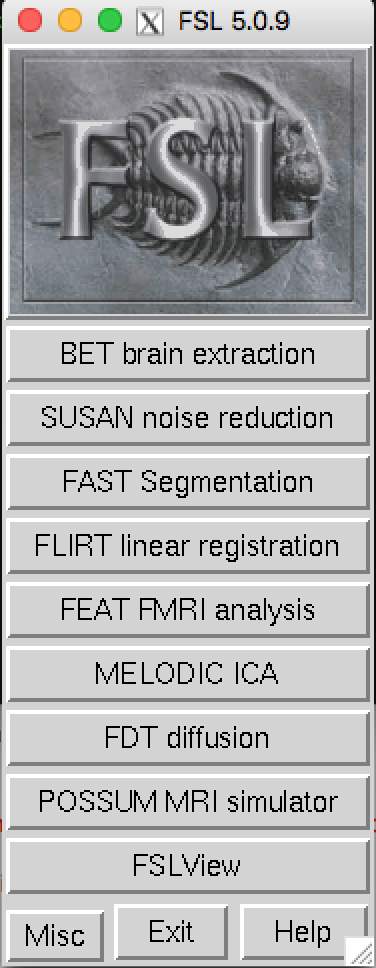
\includegraphics[width=3cm]{Figures/FSL}
    \caption{FMRIB software library user interface}
    \label{fig:fsl}
\end{wrapfigure}

\subsubsection{MRI Correction}

Bias field signal is a low-frequency, smooth signal that corrupts MRI
images due to inhomogeneities in the magnetic fields of the MRI
machine by blurring images, thereby reducing the high frequencies of
the images, such as edges and contours. The signal changes the
intensity values of image pixels so that the same tissue has a
different distribution of grayscale intensities across the
image. \cite{ref:bias} We applied an estimated bias field correction
on the $T_1$ and $T_2$ MRIs using FMRIB Software Library (FSL) FAST
\cite{ref:fslfast}, which will be further described in Section
\ref{sec:Seg}. FSL's basic user interface, which was used throughout
this pipeline, is shown in Figure \ref{fig:fsl}.

\subsubsection{DWI Distortion Correction}

DWIs performed with EPI sequences are prone to distortions from rapid switching of diffusion weighting gradients, movement from the scanning table, and movement from the subject. The diffusion data was collected with reversed phase-encode blips (anterior to posterior (AP) and posterior to anterior (PA)), resulting in pairs of images with distortions in opposite directions. From these pairs, we estimated the susceptibility-induced off-resonance field using a method \cite{ref:fsltopup1} similar to what is currently implemented in FSL.\cite{ref:fsltopup2} We then combined the two images into a single corrected one using FSL's topup and eddy command line tools.

Before running these tools, we created an acquisition parameters text file with the FSL-defined total readout time. Two parameters are frequently required to calculate and apply field maps: the effective echo spacing and the total readout time for an EPI sequence.  We used ``effective'' echo spacing, rather than the actual echo spacing, in order to include the effects of parallel imaging, phase oversampling, etc. We defined ``effective'' echo spacing as:
\[
\text{Effective Echo Spacing (s) = 1/(BandwidthPerPixelPhaseEncode * MatrixSizePhase)}
\]

The total readout time (FSL definition) was:
\[
\text{Total readout time (FSL) = (MatrixSizePhase - 1) * EffectiveEchoSpacing}
\]

The software package MRIConvert provided the acquisition information about a dicom series, as well as converted the MRI to a NiFTI format, including effective echo spacing and total readout time \cite{ref:mriconvert}. To obtain this information, we loaded the dicom series for either DWI acquisition. We selected ``Options'' to ensure the DWI was saved in NiFTI format. We then selected ``Convert All'' to save all the files into the output directory specified upon opening MRIConvert. The text file included the FSL-defined total readout time, which was contained in the acquisition parameter file in seconds. MRIConvert also output the b-values and b-vectors files, which were the same for both the DWI AP and DWI PA scans. The last input file required was an ``index.txt'' file, which contained one column with 65 rows (for 64 directions plus the b0 image) of 1's.

%MRIConvert
\begin{figure}[H]
    \centering
    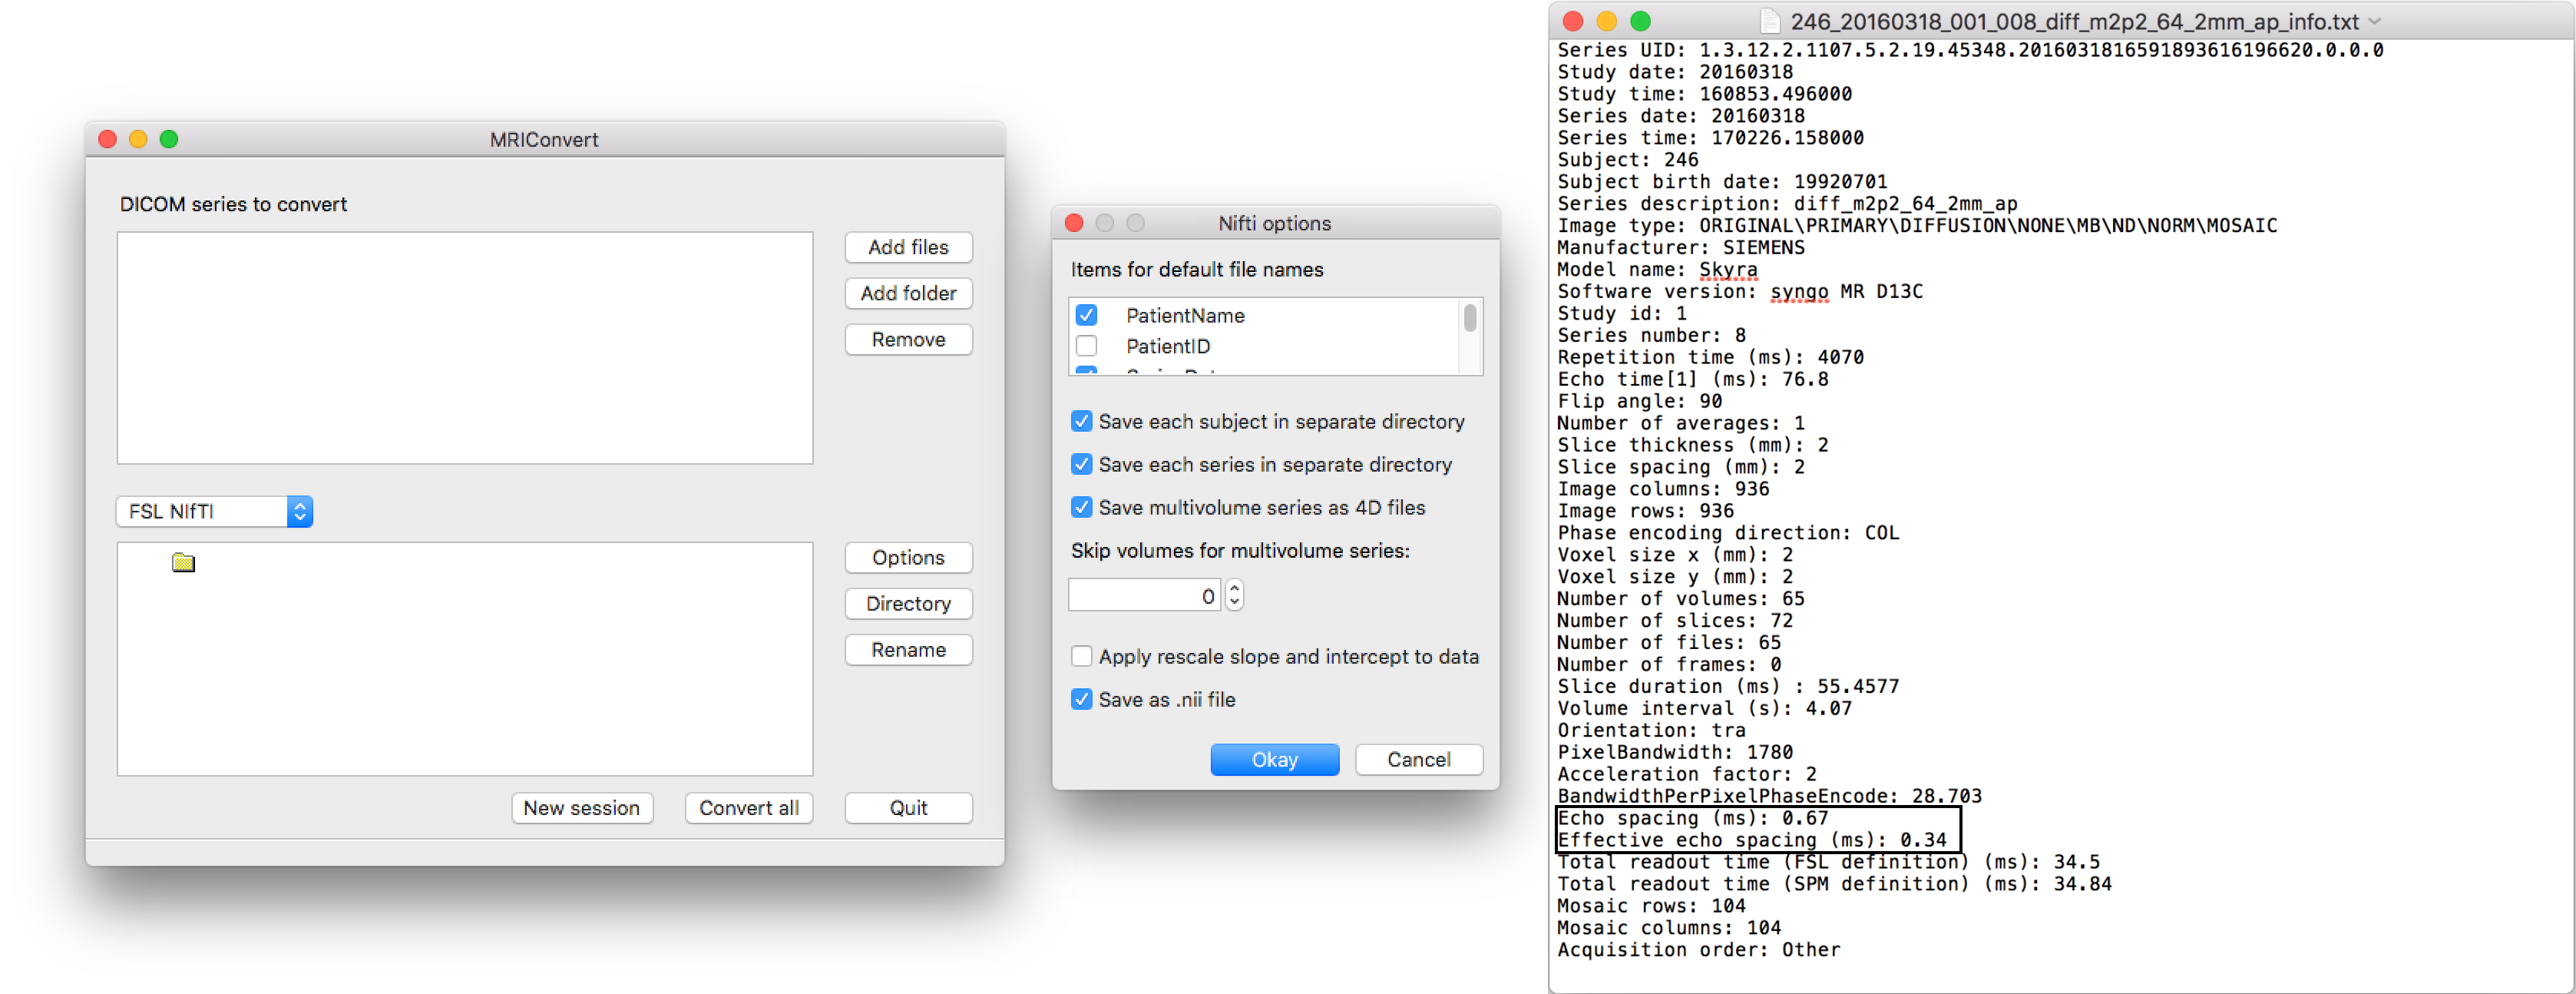
\includegraphics[width=\textwidth]{Figures/combined}
    \caption{MRIConvert \textit{(left)} with options \textit{(middle)} \& output \textit{(right)} }
    \label{fig:mri_convert}
\end{figure}

\begin{figure}[H]
\centering
{\tt
\begin{varwidth}{\linewidth}
\begin{verbatim}
0  -1 0 0.0345
0   1 0 0.0345
\end{verbatim}
\end{varwidth}
}
\label{fig:acq}
\caption{Acquisition parameters text file}
\end{figure}

We made a separate folder for topup results that included the following files: the acquisition parameters file, the index file, b-values, b-vectors, and the DWI AP and DWI PA files. To run topup, we renamed the DWI AP image DWI\_up and the DWI PA image DWI\_down. We renamed the b-values and b-vectors dwi.bval and dwi.bvec, respectively. After all files were in place, we executed the following command line commands:


\lstdefinestyle{DOS}
{
    backgroundcolor=\color{white},
    basicstyle=\scriptsize\color{black}\ttfamily
}

\begin{lstlisting}[style=DOS]
fslroi DWI\_up b0\_up 0 1
fslroi DWI\_down b0\_down 0 1

fslmerge -t both\_b0 b0\_up b0\_down

topup --imain=both\_b0 --datain=acq_params.txt --config=mine.cnf --out=topup\_results
applytopup --imain=b0\_up,b0\_down --inindex=1,2 --datain=acq_params.txt
           --topup=topup\_results  --out=b0\_hifi

bet b0\_hifi b0\_hifi\_brain -m -f 0.2
eddy --imain=DWI\_up --mask=b0\_hifi\_brain\_mask --index=index.txt --acqp=acq_params.txt
     --bvecs=dwi.bvec --bvals=dwi.bval --fwhm=0 --topup=topup\_results --flm=quadratic
     --out=eddy\_unwarped

\end{lstlisting}

By running these commands, we first obtained the b0 image, which is the baseline image used for calculating field maps, for both encoding directions. Then the two b0's were merged together into one file, topup and eddy were applied for distortion correction, and `bet' was applied for brain extraction. The distortion corrected file was named ``eddy\_unwarped.nii.''

\subsubsection{Diffusion Tensor Images}

After we corrected the DWI images, we calculated diffusion tensor images (DTI) using FSL's DTIFIT toolbox \cite{ref:dtifit}. Upon opening FSL, we chose ``FDT Diffusion,'' followed by ``DTIFIT Reconstruct diffusion tensors'' in the drop-down menu and input files manually; Table \ref{tab:dtifit} lists the files selected.

\begin{table}[H]
\centering
\caption{DTIFIT Input Files}
\label{tab:dtifit}
\begin{tabular}{|c|c|}
\hline
Diffusion weighted data & eddy\_unwarmed.nii        \\ \hline
BET binary brain mask   & b0\_hifi\_brain\_mask.nii \\ \hline
Output basename          & desired output location   \\ \hline
Gradient directions     & dwi.bvec                  \\ \hline
b values                & dwi.bval                  \\ \hline
\end{tabular}
\end{table}
DTIFIT output the eigenvalues (named L1, L2, and L3) and the eigenvectors (named V1, V2, and V3) for the diffusion tensor field. We converted the files from NiFTI format to nrrd format using ITK-SNAP \cite{ref:itksnap}, although there was a loss of precision. We then input the files into SCIRun to build the tensor field using the eigenvalue and eigenvectors. The SCIRun ``CalculateFieldData'' module requires only two eigenvectors as input because it calculates the third eigenvector automatically since it is orthogonal.

\begin{figure}[H]
\begin{center}
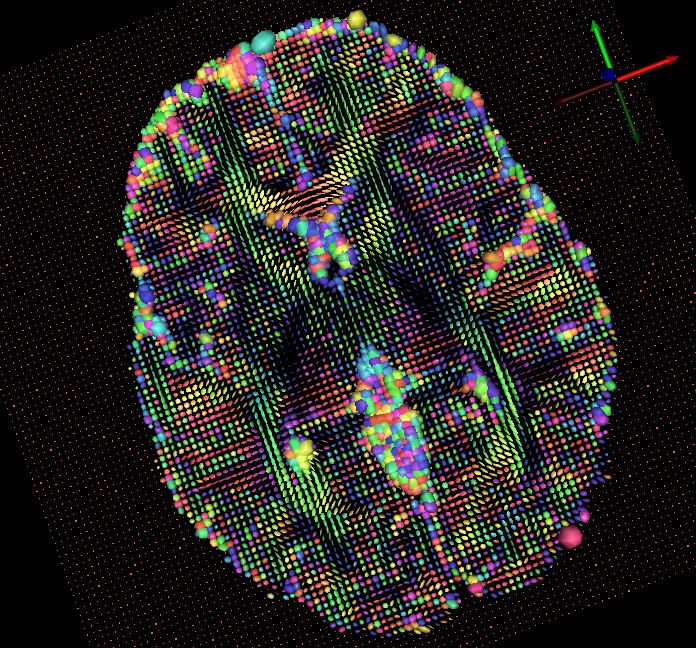
\includegraphics[width=0.75\textwidth]{Figures/DTI_1.png}
\caption{Diffusion tensor visualization using SCIRun}
\label{fig:tensorvis}
\end{center}
\end{figure}

\begin{figure}[H]
\begin{center}
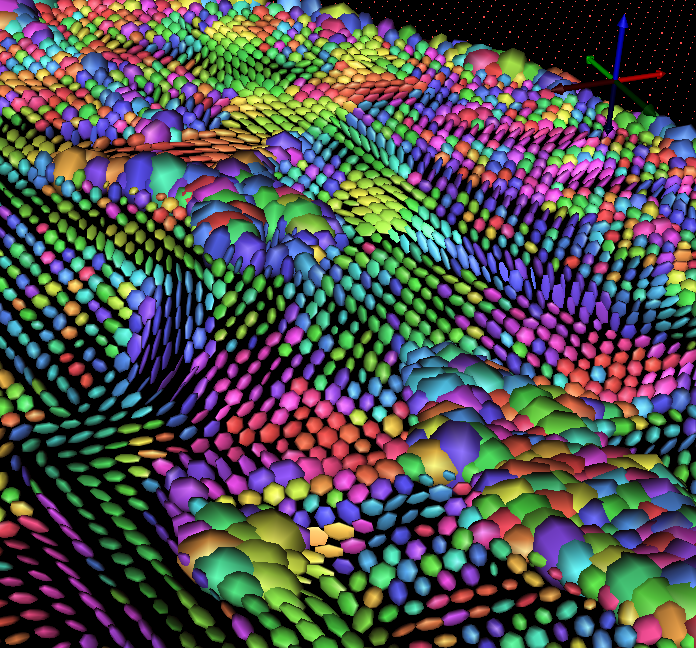
\includegraphics[width=0.75\textwidth]{Figures/DTI_2.png}
\caption{Diffusion tensor visualization using SCIRun}
\label{fig:tensorvis2}
\end{center}
\end{figure}

We built the tensor field in SCIRun rather than in 3D Slicer \cite{ref:slicer} or FSL DTIFIT because the output data had a different orientation and could not be easily registered with the mesh in SCIRun.

\begin{figure}[H]
\begin{center}
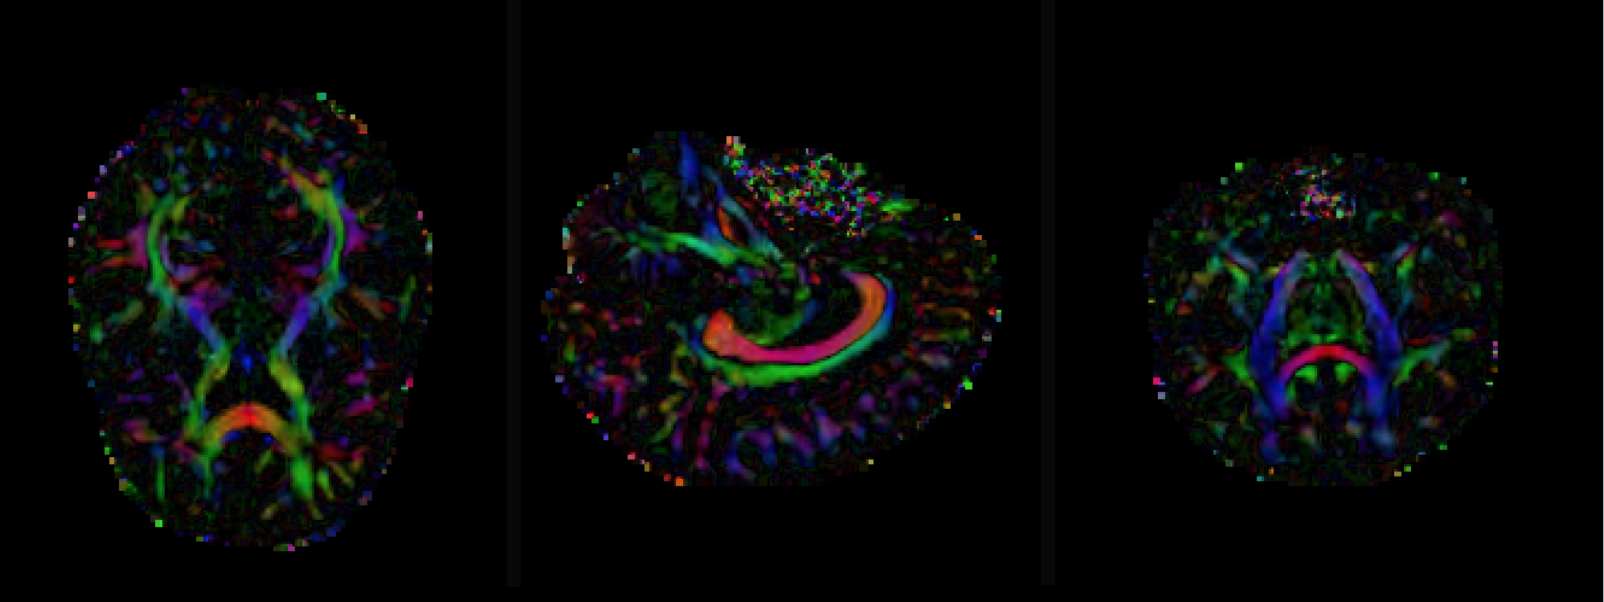
\includegraphics[width=0.75\textwidth]{Figures/backwards.png}
\caption{Example of difference in orientation between SCIRun and 3D
  Slicer data}
\label{fig:backwards}
\end{center}
\end{figure}

\subsubsection{fMRI}
\label{sec:fmripre}

We preprocessed the fMRI data using the 1000 Functional Connectomes (fcon) Project pipeline scripts \cite{ref:fcon}, which performed anatomical preprocessing, functional preprocessing, registration to the $T_1$ MRI, segmentation, and nuisance signal regress. The outline pipeline used on this fMRI dataset, specific to the University of Utah, can be found at \url{https://bitbucket.org/UtahBrainNetworks base_prep}, which includes instructions for installation, compilation, and usage.

We opened ``rest.nii,'' the preprocessed fMRI file, in Matlab using the ``load\_nii(`rest.nii')'' function within the NiFTI toolbox \cite{ref:nifti} after running the fMRI data through the fcon pipeline. We then resized the four-dimensional ``img'' variable into a two-dimensional variable for use in SCIRun.

\subsubsection{EEG}

A 60Hz notch filter and its harmonics \cite{ref:filter} were applied to the EEG data and output in .edf file format. We calculated the EEG signals matrix using a Matlab script called ``edfRead.m.'' \cite{ref:edfread} To run this script, we used ``[hdr, record] = edfread(fname).'' The variable 'record' contained the EEG signals. We removed the last two rows of the EEG signals matrix as these were control rows for the experiment. We also removed several columns at the beginning and the end of the matrix because these columns corresponded to taking the EEG net on and off the subject's head.

\subsubsection{Registration}

Since the subject did not move in between the $T_1$ and $T_2$ MRI, no registration was necessary before segmentation and meshing. We generated the tetrahedral mesh in its own coordinate space from the segmentation, and registered the mesh to the DTI coordinate space with a rigid registration using SCIRun. We registered the fMRI data to the mesh coordinate space with a rigid registration, using SCIRun as well. To register the fMRI data to the DTI coordinate space, the same transformation matrix used to register the mesh can be applied later, if desired. The SCIRun networks for registration are included in Section \ref{sec:sim}.

\begin{figure}[H]
\begin{center}
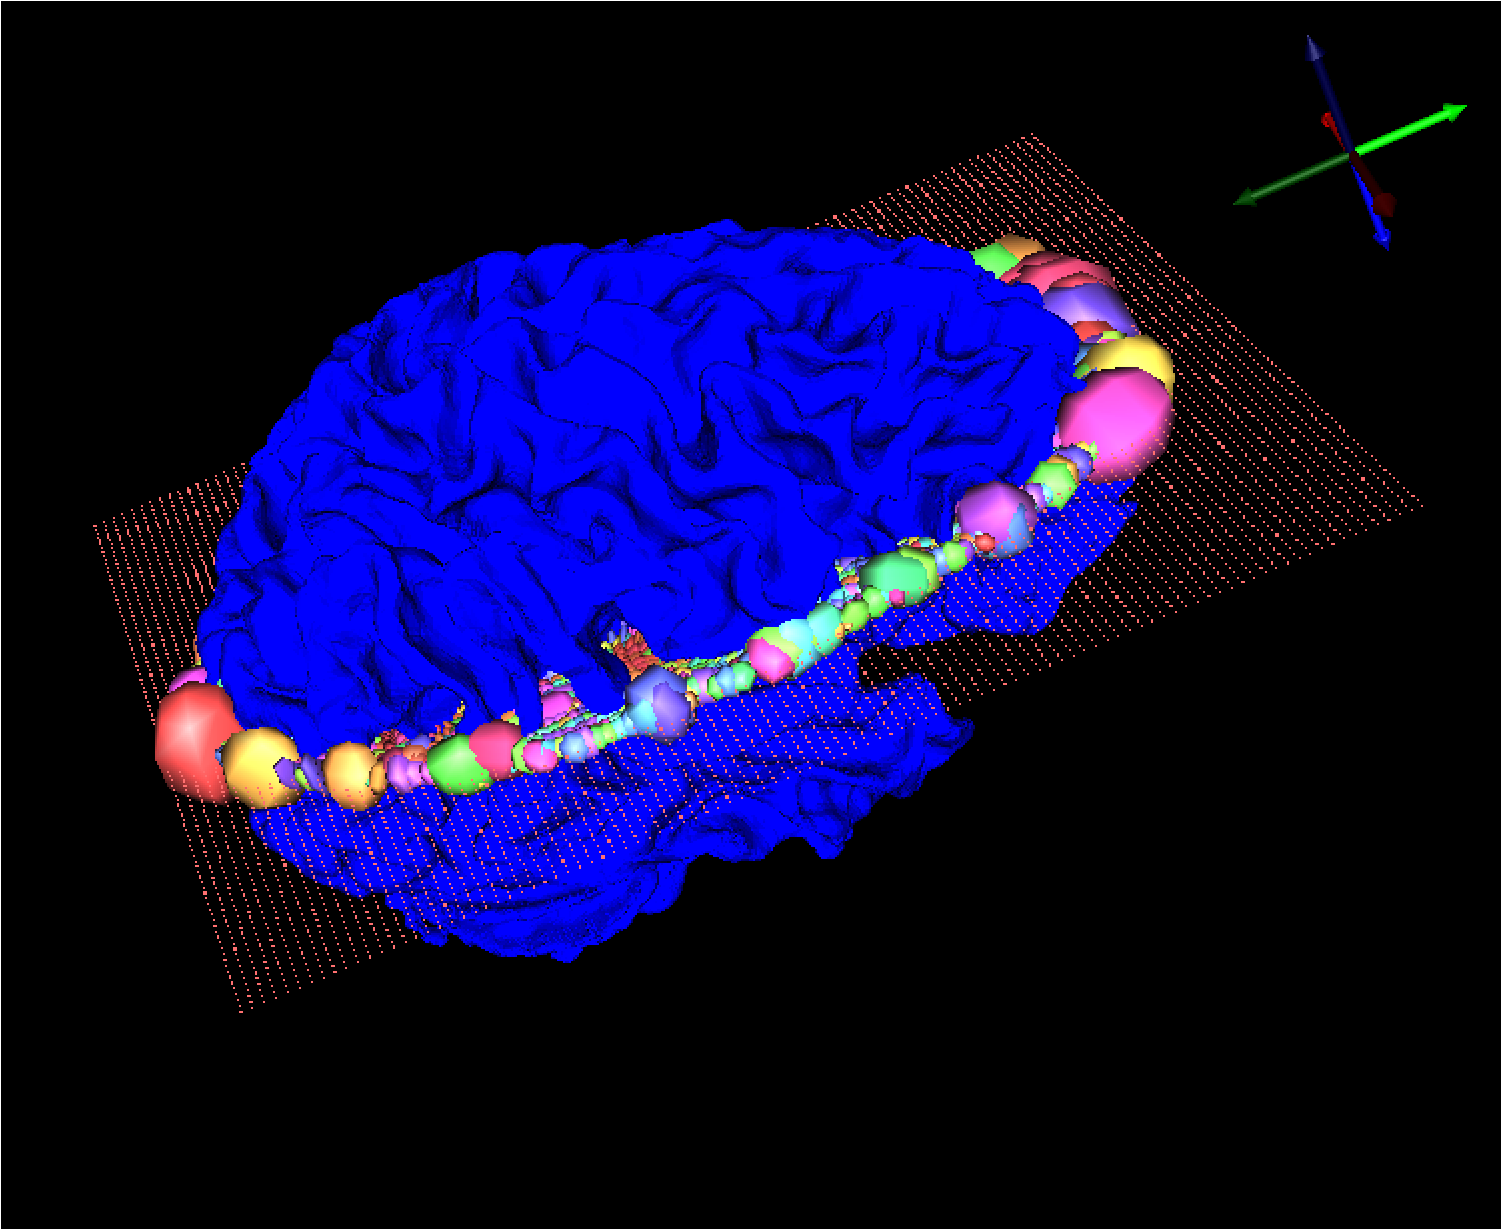
\includegraphics[height = 2.5in]{Figures/DTI_reg}
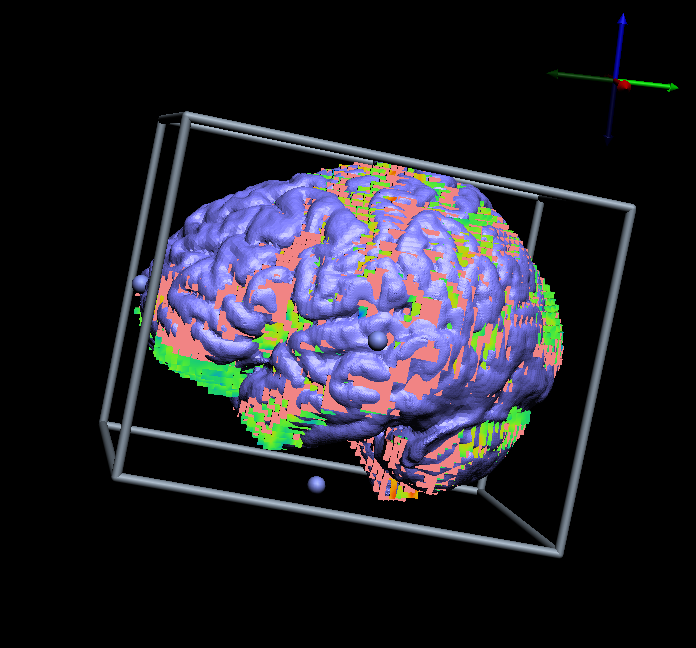
\includegraphics[height = 2.5in]{Figures/fmri_reg}
\caption{SCIRun manual registrations: mesh to DTI registration \textit{(left)}, fMRI to mesh registration \textit{(right)}}
\label{fig:dtireg}
\end{center}
\end{figure}

\subsection{MRI Segmentation of Tissues}
\label{sec:Seg}

%%% Preparation for segmentation, trials, manual work 

Segmentation of the head tissues proved to be the most time-consuming portion of the pipeline. We segmented the head volume using FSL and Seg3D, a free volume segmentation and processing tool \cite{ref:seg3d} into air, cerebral spinal fluid (CSF), white matter, gray matter, skull, sinus, eyes, and scalp. Segmentation of the brain was difficult due to the similar grayscale intensities across different tissues; thresholding the image produced noisy and incomplete layers. Segmentation of the sinuses and skull was also difficult because they are represented by only black pixels, with no clear tissue boundaries.

We initially segmented the brain by inputting a skull stripped $T_1$ MRI into FSL FAST Segmentation. We skull stripped the $T_1$ MRI using FSL's brain extraction tool (BET) \cite{ref:bet1}. FSL FAST outputs segmented CSF, white matter, and gray matter layers as well as a bias-corrected $T_1$ MRI. This method, compared with Freesurfer \cite{ref:freesurf}, Statistical Parametric Mapping through Matlab (SPM) \cite{ref:spm}, Atlas Based Classification through 3D Slicer \cite{ref:abc}, and Seg3D methods alone, produced the best initial brain segmentation results for this data.
\begin{figure}[H]
    \centering
    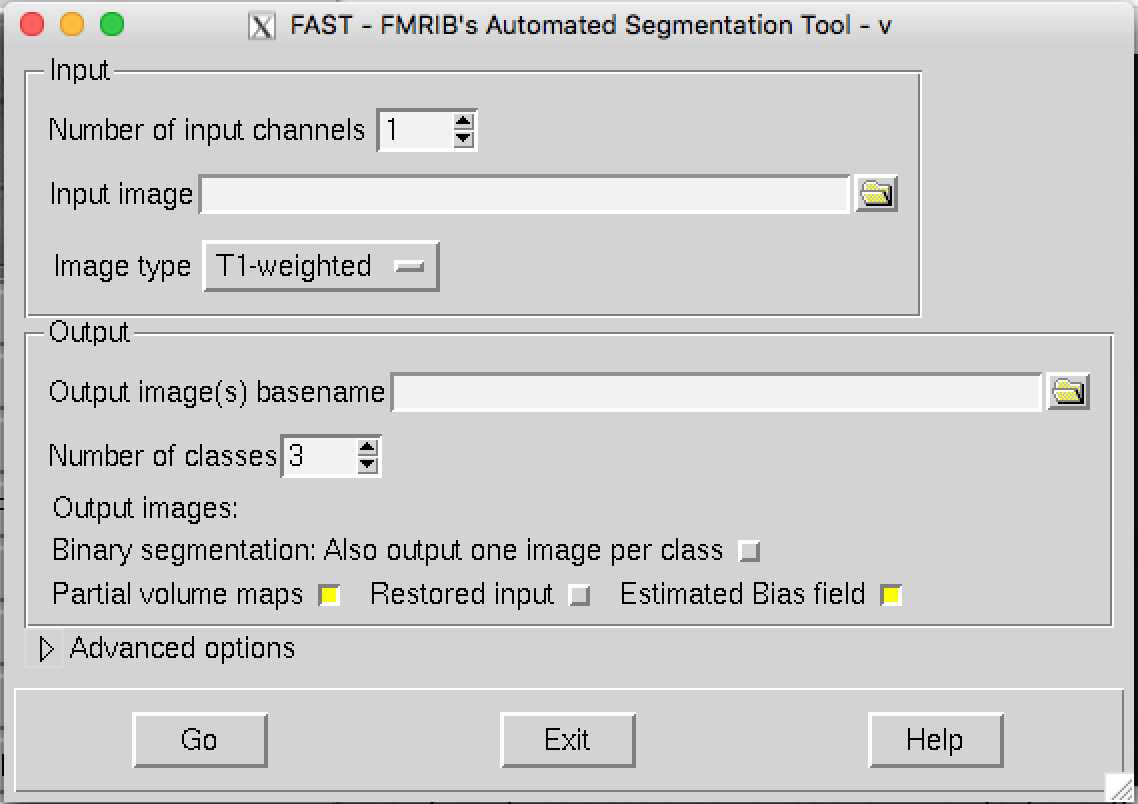
\includegraphics[width=.8\textwidth]{Figures/FSL_FAST}
    \caption{FSL FAST user interface}
    \label{fig:fslfast}
\end{figure}

\begin{figure}[H]
\begin{center}
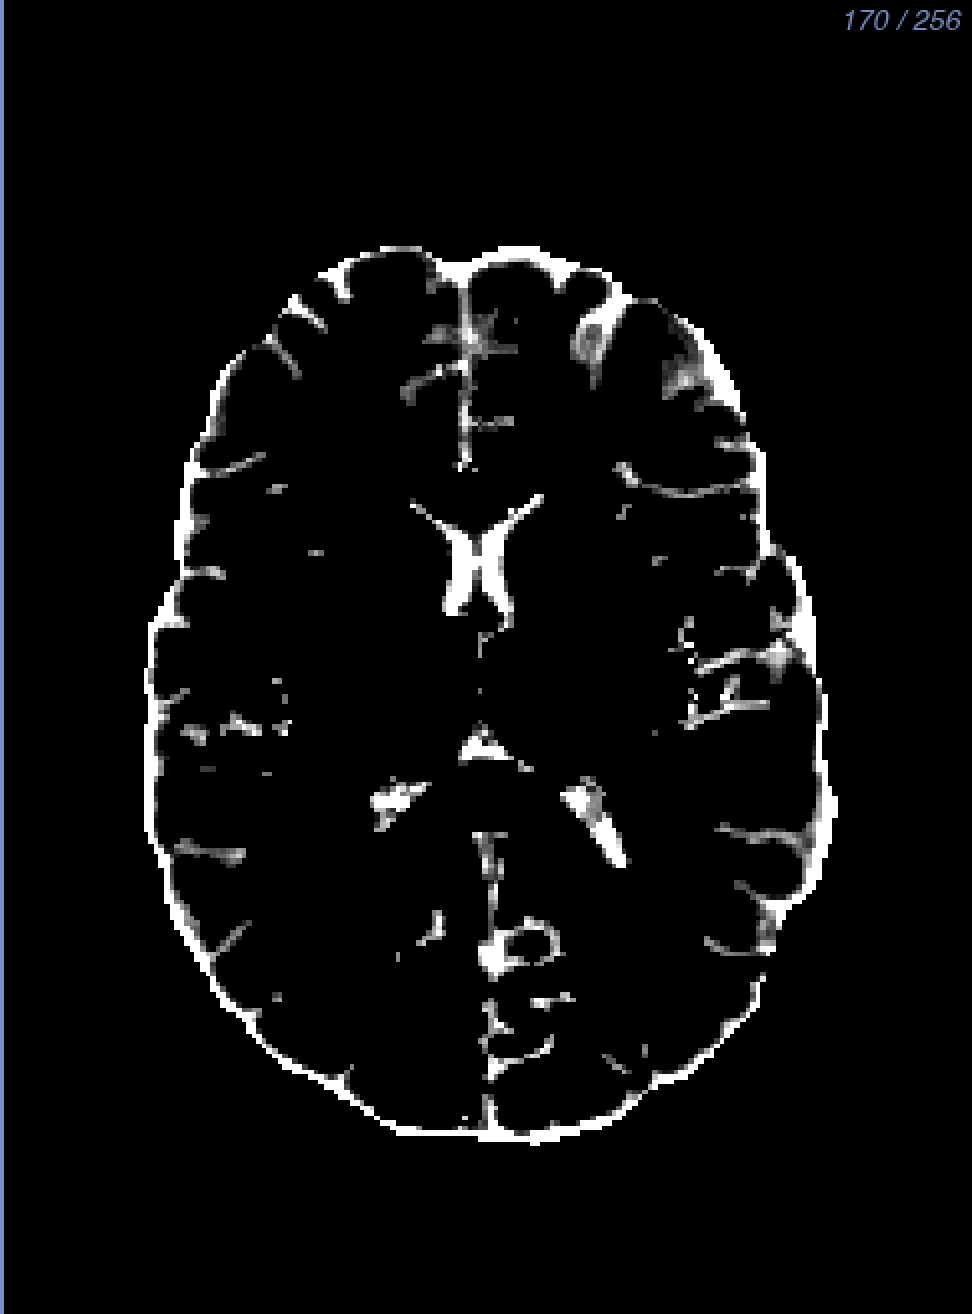
\includegraphics[width=.32\textwidth]{Figures/FSLFAST_csf}
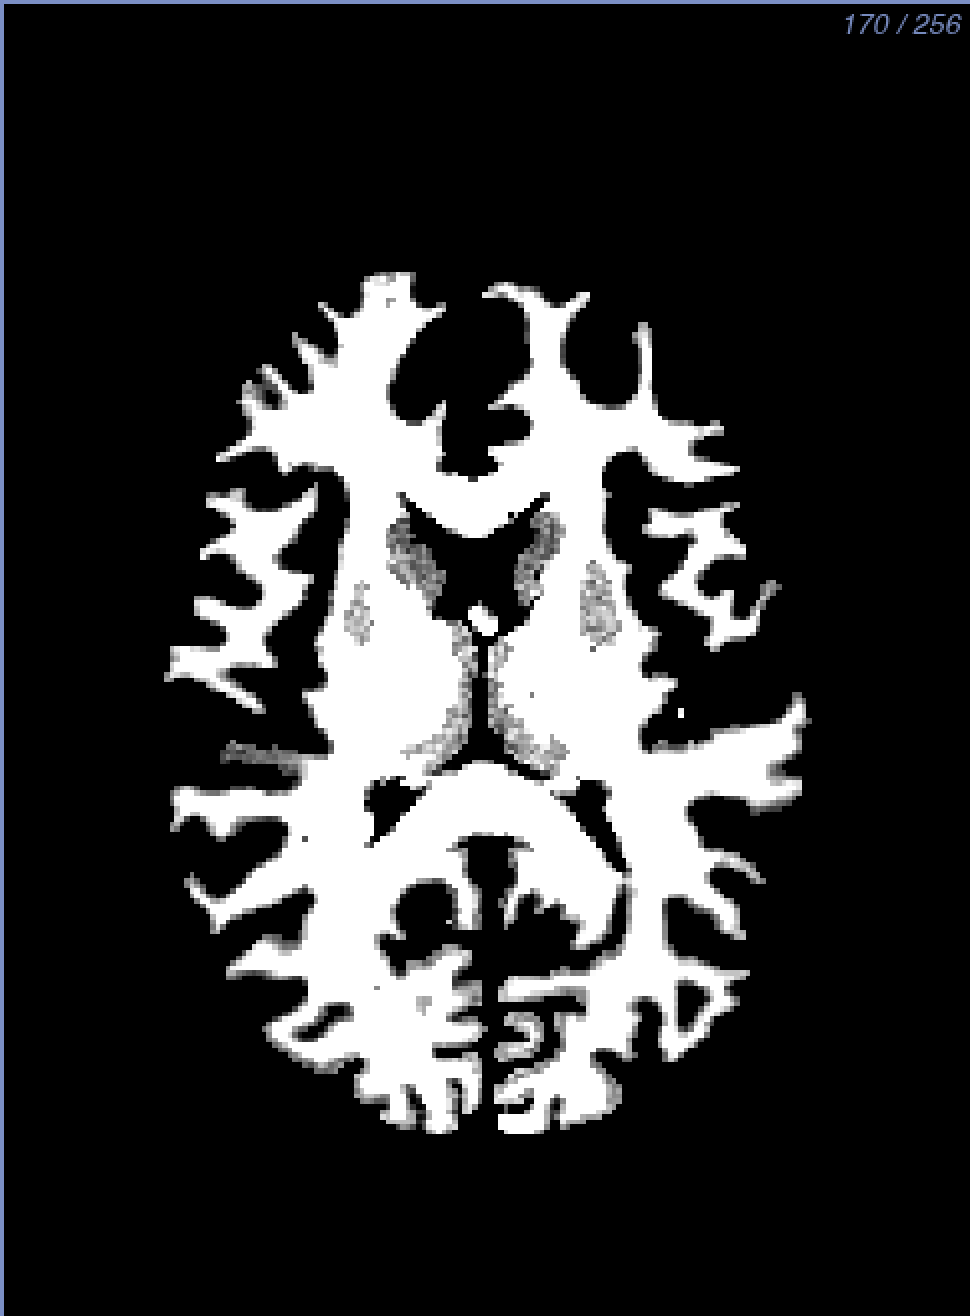
\includegraphics[width=.32\textwidth]{Figures/FSLFAST_wm}
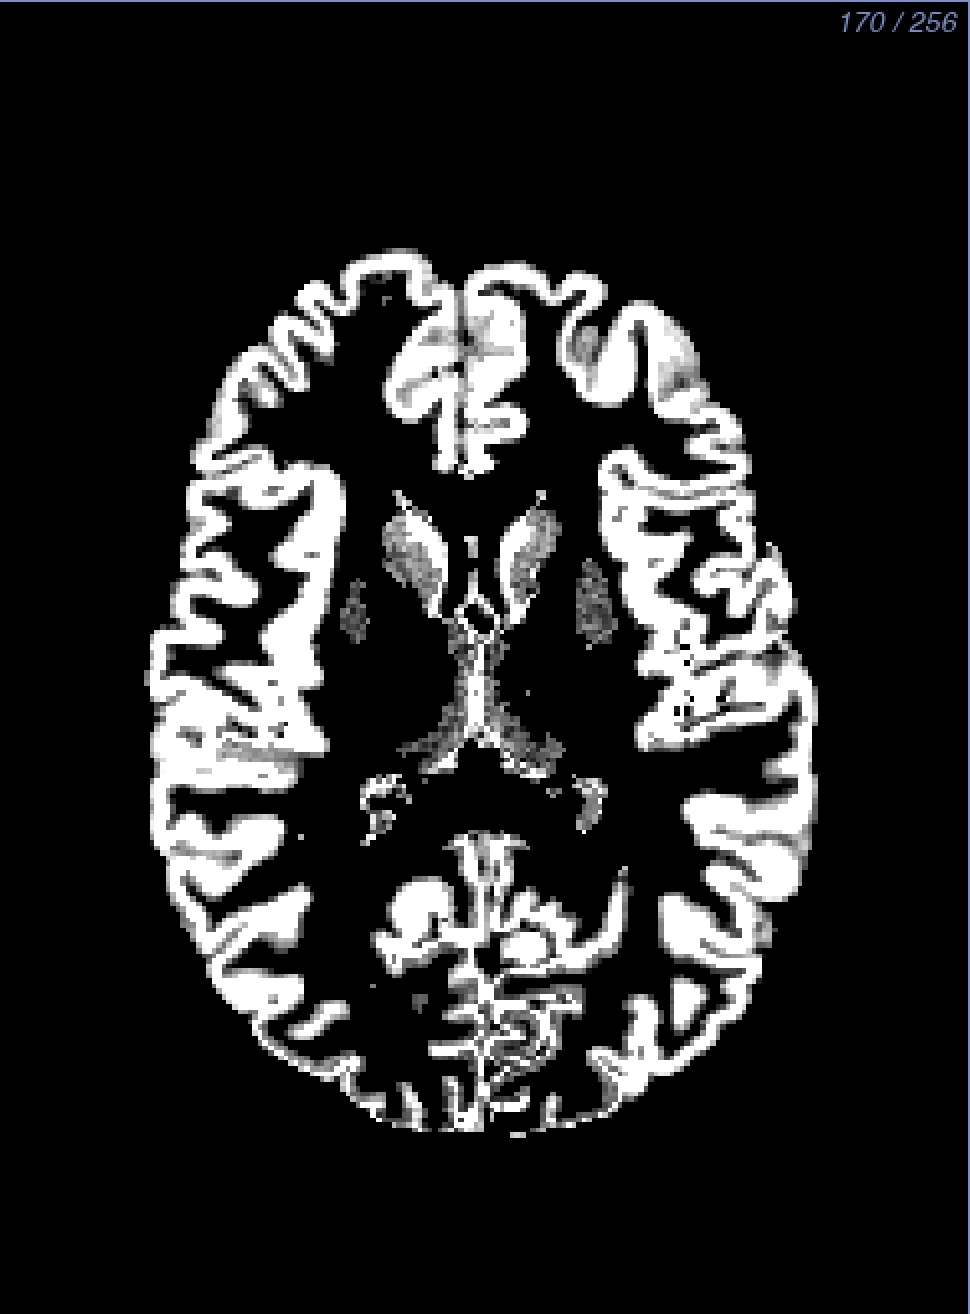
\includegraphics[width=.32\textwidth]{Figures/FSLFAST_gm}
\caption{FSL FAST output: CSF \textit{(left)}, white matter \textit{(center)}, gray matter \textit{(right)}}
\label{fig:fastout}
\end{center}
\end{figure}

Although the FSL FAST results were an improvement compared to the other segmentation software trials, we manually improved the layers to add more detail and to remove any crossover between the layers. We started with the white matter layer because it is the innermost layer. First, we created a threshold layer FSL FAST output. We then inspected and manually edited each slice in every direction to add more detail or to clean up noise from FSL FAST.

\begin{figure}[H]
\begin{center}
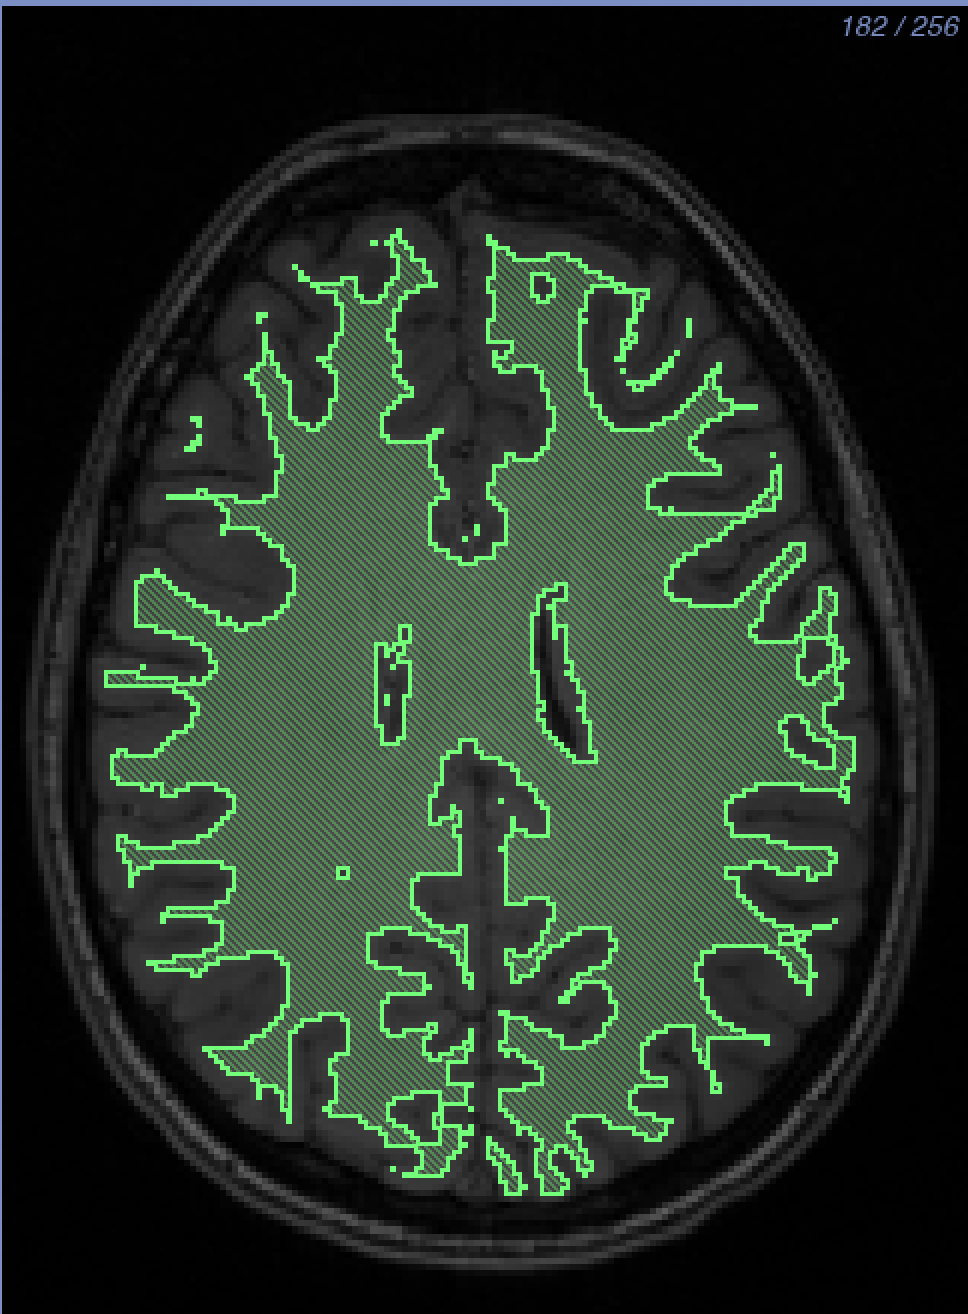
\includegraphics[width=.49\textwidth]{Figures/whitematter_before}
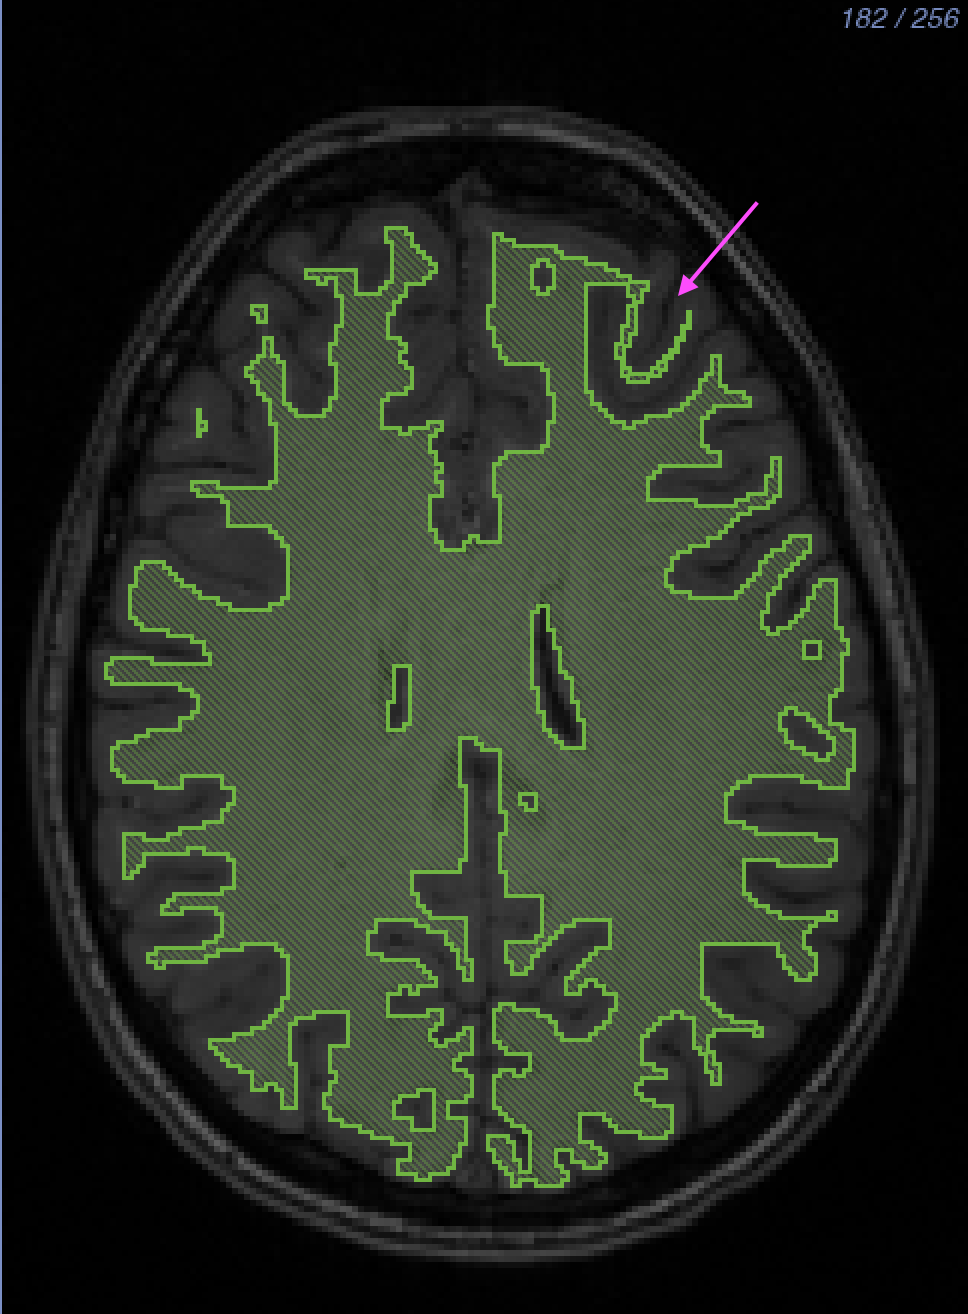
\includegraphics[width=.49\textwidth]{Figures/whitematter_after}
\caption{White matter segmentation: Before \textit{(left)} and after \textit{(right)} manual segmentation. The hook feature in the upper right-hand corner is a notable change between the two layers. The layer is more full and has less noise.}
\label{fig:wm}
\end{center}
\end{figure}

After we segmented the white matter, we created a threshold layer from the FSL FAST output for the gray matter. We inspected and manually edited each slice in every direction of the gray matter. We then removed the white matter layer from the gray matter using a Boolean remove mask filter to ensure no overlap between the layers. We manually filled any holes between the two layers. Lastly, we added a gray matter nuclei to the gray matter layer. The thresholding algorithms in Seg3D produced noise around these nuclei because of the similarities of the grayscale values. To fix this noise, we segmented the entire nuclei manually using the paintbrush tool in Seg3D. Then, we added the nuclei to the gray matter layer using a Boolean OR mask filter, and removed any overlap from the white matter layer using a Boolean remove mask filter.

\begin{figure}[H]
\begin{center}
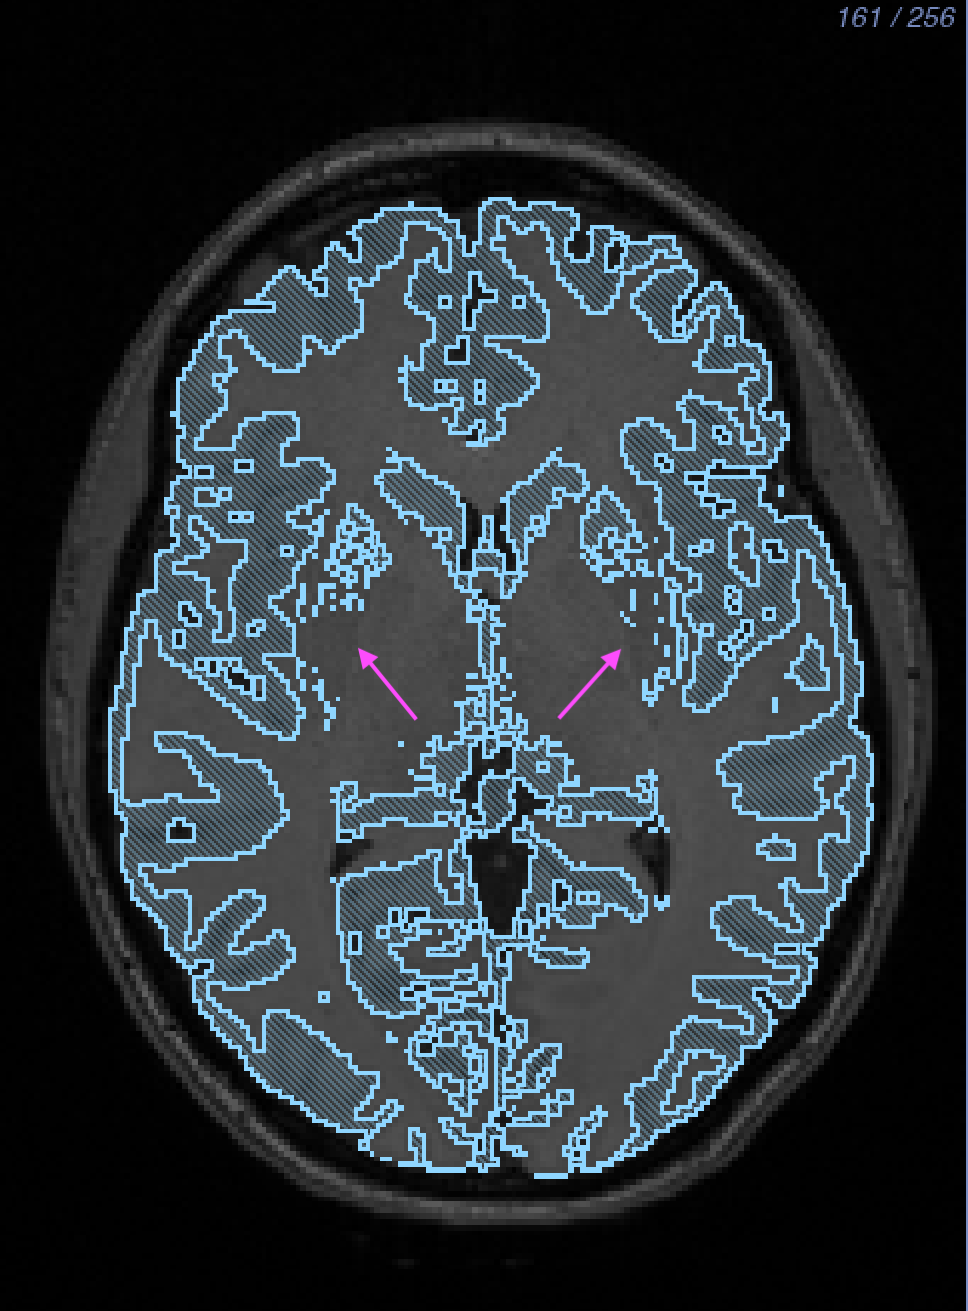
\includegraphics[width=.49\textwidth]{Figures/greymatter_before_nuclei}
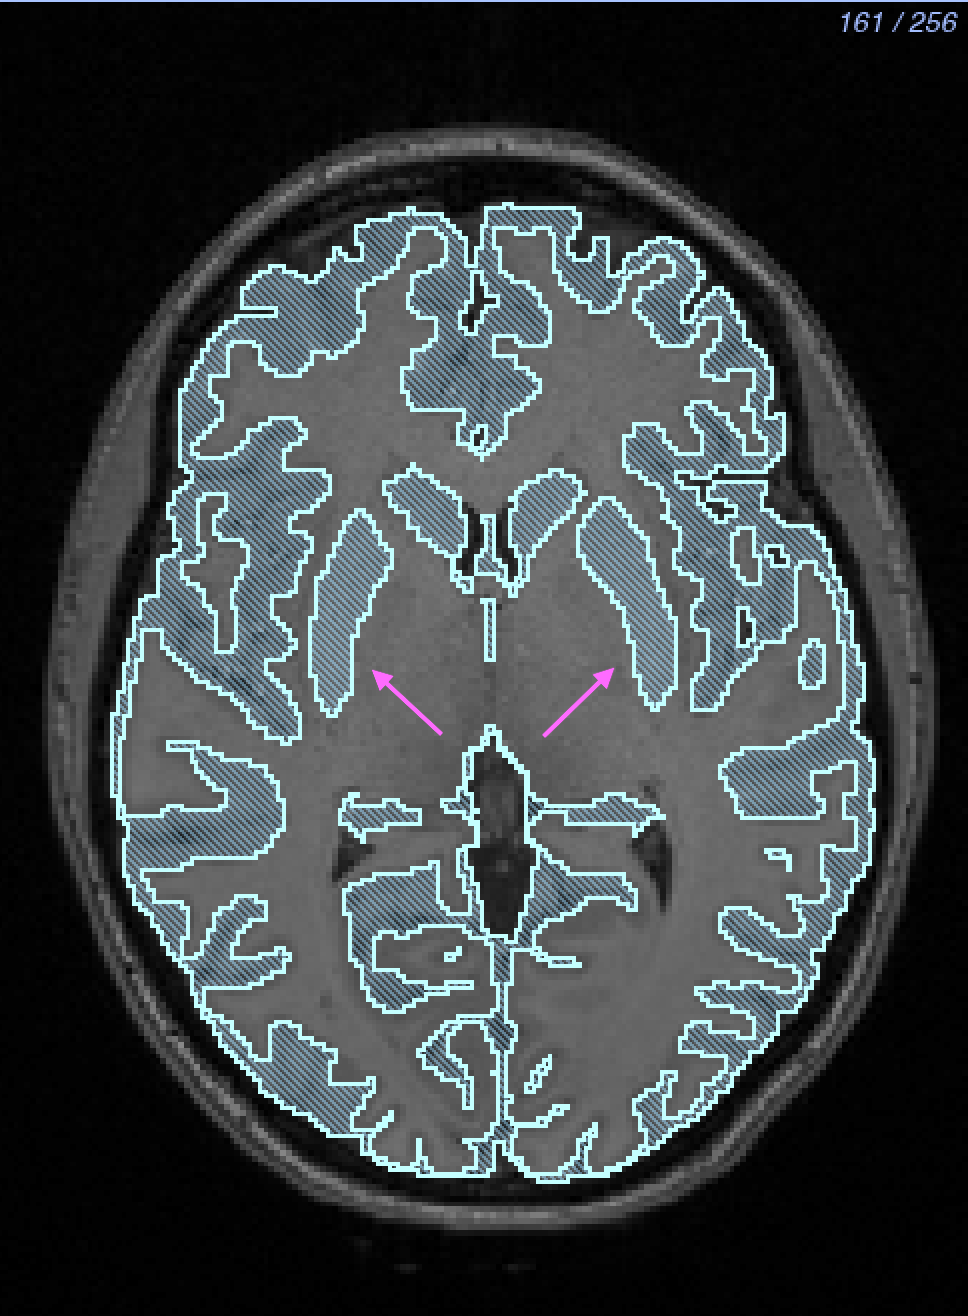
\includegraphics[width=.49\textwidth]{Figures/greymatter_added_nuclei}
\caption{Gray matter segmentation: Before \textit{(left)} and after \textit{(right)} manual segmentation. Gray matter nuclei located in the center of the brain were segmented manually.}
\label{fig:gm}
\end{center}
\end{figure}

After we completed the segmentation of the gray and white matter layers, we made the CSF layer by creating a solid threshold layer for the entire brain and removing the white and gray matter layers using a Boolean remove mask filter. We then checked the white matter, gray matter, and CSF layers for holes, both on the surface and inside the segmentation between layers. We also performed a quality check on the layers to ensure that they were at least two pixels wide throughout. We chose this check to help create a tetrahedral mesh without holes.

\begin{figure}[H]
\begin{center}
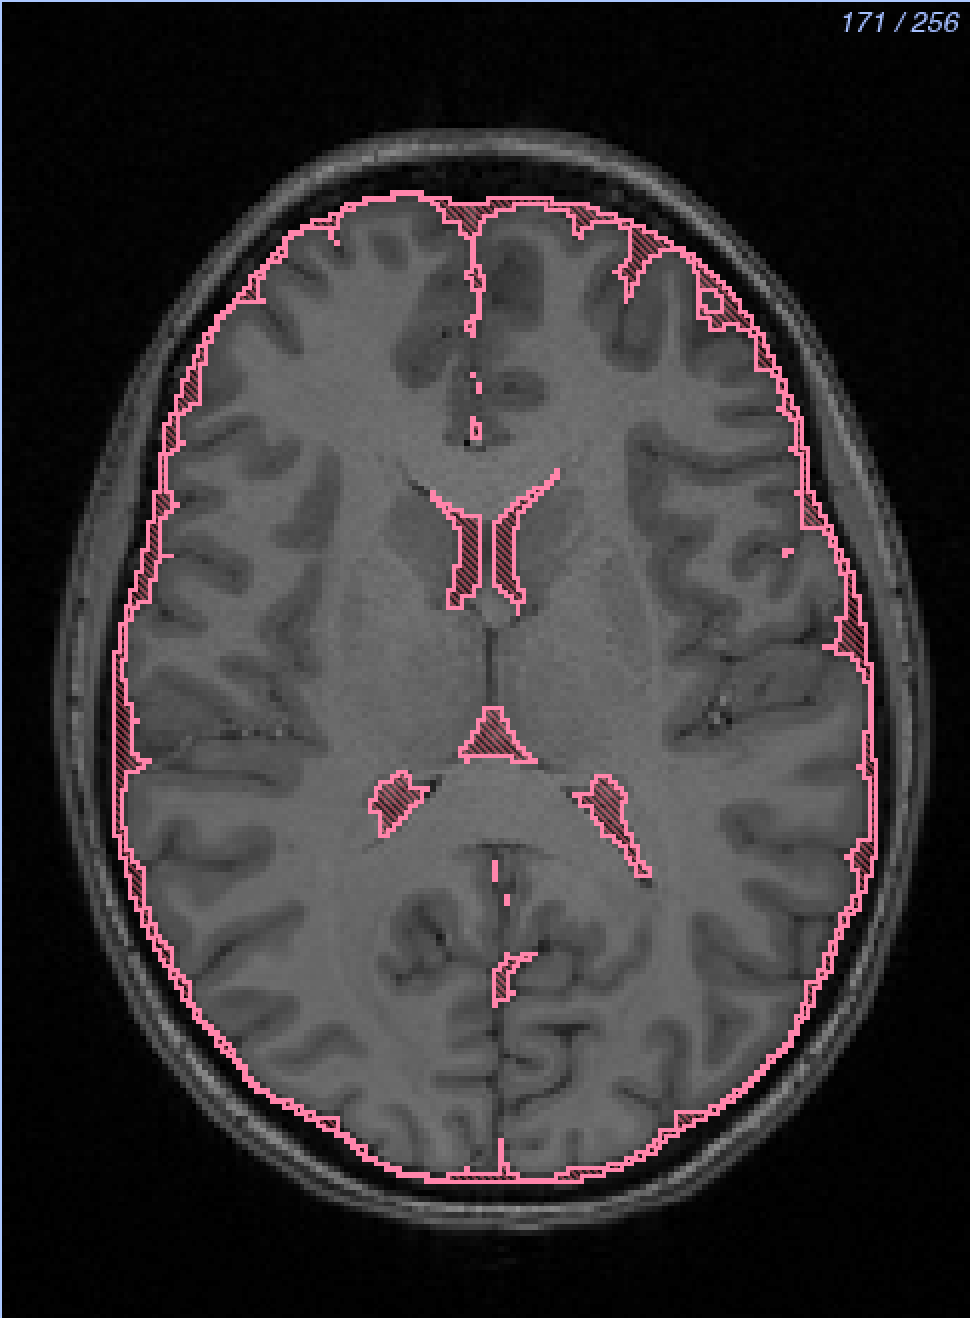
\includegraphics[width=.49\textwidth]{Figures/CSF_seg}
\caption{CSF segmentation}
\label{fig:csf}
\end{center}
\end{figure}

The skull and the sinus layers were the most difficult to segment using only an MRI because they both appear black in the MR image, and the subject's data did not include a computed tomography (CT) scan. Our first attempt to create a bone layer applied FSL's skull stripping function by using the BET2 tool to create a skull. We then thresholded the $T_1$ MRI to create the remainder of the bones in Seg3D and connected the bones to the skull made from FSL. Although this approach gave an adequate skull segmentation considering we had only an MR image, our method for segmenting the sinus layer was yet to be determined. As a second method, we estimated the skull from an MR-based synthetic pseudo-CT. We used an improved iterative version of the patch-based method as described by Torrado-Carvajal et al. \cite{ref:pseudoct} that takes the $T_1$ and $T_2$ images as input and synthesizes the pseudo-CT based on both images, providing more refined and accurate bone boundaries.

\begin{figure}[H]
\begin{center}
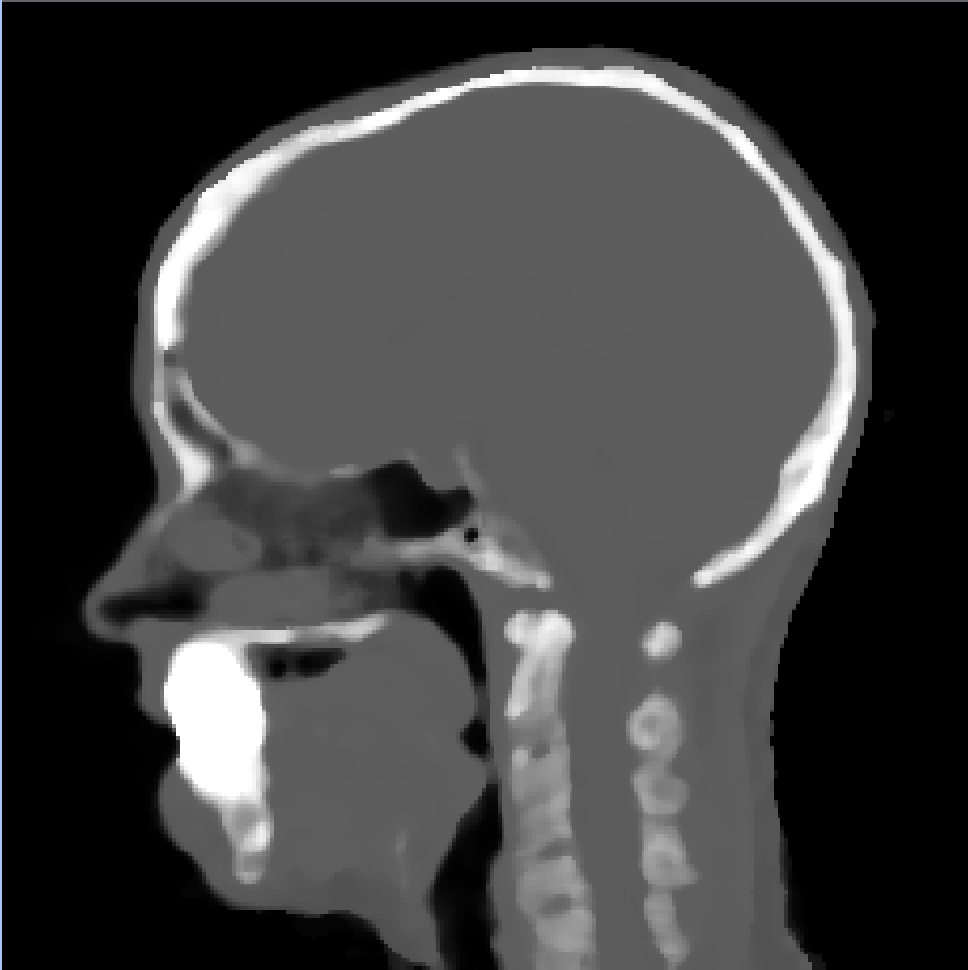
\includegraphics[width=.75\textwidth]{Figures/pseudo_CT}
\caption{Pseudo-CT scan}
\label{fig:ct}
\end{center}
\end{figure}

The pseudo-CT method provided an image that was an easier starting place for skull segmentation, but we still manually edited the layer to add detail. After we applied a median filter with a one-pixel radius and thresholded the skull segmentation, we manually edited each slice in every direction to add detail and to smooth noisy sections of the layer. Since the subject had a permanent retainer in her mouth that created all black pixels, we segmented the mouth as solid bone, which was not concerning because the EEG cap used did not cover the subject's mouth. We were able to provide a segmentation of the internal air, including the sinuses, esophagus, and ear canals, from the pseudo-CT image by thresholding the black pixels and then manually editing each slice. We also performed a quality check on both layers to ensure they had no holes or layer overlap and that they were at least two pixels thick.

The eyes, skin, and air layers were the least time consuming to segment. We segmented the eyes by thresholding the $T_2$ MRI. We segmented the skin layer by thresholding the entire head volume and removing all previous layers using a Boolean remove mask filter. We performed a quality check on the skin layer to ensure that it was at least two pixels thick. The important places for the quality check are the bridge of the nose, the bottom of the chin, and the sides of the head. Lastly, we segmented the air layer by thresholding the entire image and removing the solid skin layer, followed by a check to ensure that the segmentation did not contain any holes between layers after they were removed. This final step is imperative to assure a quality mesh.

\begin{table}[H]
\centering
\caption{Segmentation Time}
\label{tab:seg}
\begin{tabular}{|c|c|}
\hline
Segmented Tissue    & Amount of Work (hrs) \\ \hline
White Matter       & 40                   \\ \hline
Gray Matter         & 20                   \\ \hline
CSF                 & 4                    \\ \hline
Skull and Sinus     & 35                   \\ \hline
Eyes, Scalp, \& Air & 8                    \\ \hline
\end{tabular}
\end{table}

\subsection{Finite Element Mesh Generation}
\label{sec:mesh}

%%% Settings for mesh generation, issues 

We used our full-head segmentation to generate realistic three-dimensional geometries for use in subsequent finite element simulations. We generated a smooth, linear, subject-specific, boundary-conforming, tetrahedral finite element mesh using the Cleaver software \cite{ref:cleaver} on a Late 2013 Mac Pro with a 2.7 Ghz 12 Core Intel Xeon E5 processor with 64 GB of RAM and an AMD FirePro graphics card. Cleaver is a multi material meshing package that produces structured meshes of tetrahedral elements with guaranteed minimum element angles, resulting in quality meshes that require fewer computational resources. We made a high-resolution mesh without holes using the parameters listed in Table \ref{tab:cleaver}.
\begin{table}[H]
\centering
\caption{Clever Settings (High Resolution)}
\label{tab:cleaver}
\begin{tabular}{|c|c|}
\hline
scaling factor                    & 0.6                 \\ \hline
size multiplier                   & 1.0                 \\ \hline
lipschitz                         & 0.2                 \\ \hline
padding                           & 0                   \\ \hline
element sizing method             & adpative            \\ \hline
\end{tabular}
\end{table}

Along with these parameters, indicator functions had to be input into Cleaver. We created indicator functions by calculating inverted distance maps of each layer in the full-head segmentation in Seg3D. To reduce the size of the mesh we first generated a new mesh, changing only the scaling factor parameter to 1.0 from the parameters in Table \ref{tab:cleaver}. We exported the computing sizing field from Cleaver and manipulated it in SCIRun by changing how quickly the elements increased in size. We input the changed sizing field into Cleaver with the same indicator functions and successfully cleaved a new, smaller mesh without holes.

\subsection{Mathematical Modeling}
\label{sec:math}

%%%MATH

We used the head mesh, with associated inhomogeneous and anisotropic regions, as a volume conductor to solve the following boundary value problem:
%
\begin{equation}
\label{eq:1} \nabla\cdot\sigma\nabla\Phi = -I_{V} \;\;\;\;\mbox{ in
}\Omega,
\end{equation} 
%
where $\Phi$ is the electrostatic potential, $\sigma$ is the electrical conductivity tensor, and $I_{V}$ is the current per unit volume defined within the solution domain, $\Omega$. Equation \ref{eq:1} was solved for $\Phi$ with a known description of $I_{V}$ and the Neumann boundary condition:
%
\begin{equation} \sigma\nabla\Phi\cdot{\bf
n} = 0\;\;\;\;\;\mbox{ on }\Gamma_{T}, 
\end{equation} 
%
which says that the normal component of the electric field is zero on the surface interfacing with air (here denoted by $\Gamma_{T}$). The brain and surrounding tissue and skull were discretized using dipoles for the current source. We calculated the electrical field within the brain and then projected the field onto the surface of the scalp. \cite{ref:math}

\subsubsection{Electrical Conductivity Preparation}
\label{sec:cond}

All electrical conductivities were homogeneous for each tissue with the exception of the white matter when using tensor data. The isotropic conductivities \cite{ref:cond} we used are shown in Table \ref{tab:cond}.

\begin{table}[H]
\centering
\caption{Isotropic Tissue Conductivity}
\label{tab:cond}
\begin{tabular}{|c|c|}
\hline
Tissue Type               & Isotropic Conductivity $(S/m)$ \\ \hline
\hline
White Matter              & 0.1429                         \\ \hline
Gray Matter               & 0.3333                         \\ \hline
Cerebrospinal Fluid (CSF) & 1.79                           \\ \hline
Skull                     & 0.001                          \\ \hline
Skin                      & 0.4346                         \\ \hline
Sinus                     & 1e-6                           \\ \hline
Eyes                      & 0.5051                         \\ \hline
\end{tabular}
\end{table}

When we added the DTI tensor data, we used two approaches to convert the tensor data to conductivities. The first was scaling the data \cite{ref:scaling}: 

\begin{equation}
\label{eq:scaling}
\sigma_{aniso} = \frac{\sigma_{iso}}{\sqrt[3]{d_1d_2d_3}}D,
\end{equation}
where $D$ is the diffusion data, $d_i$ is the $i$th eigenvalue of $D$, and $\sigma_{iso}$ is the white matter isotropic conductivity. The second method gave the white matter a fixed ratio of conductivity:

\begin{equation}
\label{eq:fixed}
\sigma_{aniso} = \begin{bmatrix}
v_1\\
v_2\\
v_3\\
W\\
\end{bmatrix}, 
W = \begin{bmatrix}
\sigma_{iso}\\
\frac{\sigma_{iso}}{10}\\
\frac{\sigma_{iso}}{10}\\
\end{bmatrix},
\end{equation}
where $v_i$ is the $i$th eigenvector of $D$, $W$ is the white matter ratio vector, and the ratio is $10:1$.

\subsubsection{Numerical Methods}
\label{sec:numerical}

%%% This paragraph addresses Finite Element Discretization

We computed solutions to Equation \ref{eq:1} using finite element methods.  By applying 
Green's divergence theorem to Equation \ref{eq:1}, we generated the following weak formulation:
\begin{equation}
\int ((\bar{\sigma}_e + \bar{\sigma}_i)\nabla \phi_e) \cdot \nabla \psi(\bar{x})d\bar{x} = - \int (\bar{\sigma}
_i \nabla V_m)\cdot \nabla \psi(\bar{x})d\bar{x}, \quad \quad \forall \ \psi \in \Omega
\label{eq:galerkin}
\end{equation}
where $\Omega$ is the linear, finite element mesh, and $\psi$ represents the finite element basis functions characterized by local hat functions associated with mesh nodes. By applying this formulation to the finite-dimensional mesh, we reduced Equation \ref{eq:galerkin} to a system of linear equations:
\begin{equation}
A \phi_e = -RV_m,
\label{eq:ReducedFormula}
\end{equation}
where $A$ and $R$ represent stiffness matrices defined by $A_{j,k} = \langle \nabla \psi_j,(\bar{\sigma}
_e + \bar{\sigma}_i)\nabla \psi_k \rangle_\Omega$ and $R_{j,k} = \langle \nabla \psi_j,\bar{\sigma}_i
\nabla \psi_k \rangle_\Omega$,
and $\phi_e$ and $V_m$ represent extracellular and transmembrane potentials, respectively.\cite{ref:fem}

%%% This paragraph addresses SCIRun as a solver
We used SCIRun, the open-source problem-solving environment, to apply parameters and to solve Equation \ref{eq:ReducedFormula} numerically.  Within the SCIRun environment, we applied isotropic and anisotropic conductivity tensors to the tetrahedral mesh as well as to inhomogeneous regions. We defined initial and boundary conditions and generated border regions in order to compute potentials by way of a conjugate gradient method with a Jacobi preconditioner.

\subsection{Simulations and Visualizations}
\label{sec:sim}

We ran all simulations and visualizations in the SCIRun problem-solving environment. All networks are shown in Figures \ref{fig:maketensornet} - \ref{fig:eegvisnet}.

\subsubsection{Forward Problem}

Solving systems from a known source to the EEG electrodes, described in Section 2.5, is known as a forward problem. The opposite action, solving systems from the EEG data to a unknown source, is an inverse problem.  In this project, we built SCIRun networks to solve forward problems with known sources and to write a lead field matrix for inverse problem networks in the future. We solved forward problems with an isotropic and anisotropic conductivities, using iDTI data for the direction for anisotropic conductivities.

The necessary network inputs for the isotropic case were the tetrahedral head mesh, isotropic conductivities, the head segmentation, the physical electrode locations, and dipole sources. The physical electrode locations and the dipole sources were results from the EEG recording dataset, and contained 4800 dipoles and 256 electrodes. The network removed the fiducials from the electrode locations, and allows the user to choose a dipole source from the dataset. We registered the mesh to the head segmentation using a rigid registration. After we cut the flat tetrahedra out of the mesh, we mapped the conductivities to their respective tissues. We registered the electrodes and dipoles to the head mesh using the same transform. We solved the system with the mapped data and the chosen dipole sources. We then mapped the solution onto the mesh and the electrodes for visualization. We also included streamlines and isolines in the visualization.

For the anisotropic case, the network was largely the same with the exception of the scaled diffusion tensor dataset used as white matter conductivities. In addition, the DTI to mesh transform was needed as input. We registered the head mesh, electrodes, and dipoles to the DTI space with a rigid registration; the head segmentation was not needed.

\subsubsection{fMRI}

We visualized the fMRI data one step at a time using the two-dimensional matrix described in Section \ref{sec:fmripre} as input and viewed one column at a time. We set each column onto a lattice volume, rotated it 180 degrees, smoothed, thresholded, and clipped the volume for easier rigid registration. We registered the fMRI to the tetrahedral mesh using the bounding boxes and manual registration. After registration, we mapped the smoothed fMRI data onto the mesh using a mapping matrix with a linear interpolation basis.

\subsubsection{EEG}

We visualized the EEG data on the physical electrode locations, which we registered to the mesh space with a rigid registration after removing the fiducials from the electrode dataset. We used the filtered and cut EEG matrix as input and represented each time step as a column. We then placed the electrodes onto the mesh and mapped the EEG data onto the electrodes one time step at a time.